%% stripped down version of "bare_jrnl.tex" for use in Casey's Circuits I class.
%% Original version has very good comments for use. You should check it out at
%% http://www.ieee.org/publications_standards/publications/authors/authors_journals.html
%% I run GNU/Linux so I downloaded the "Unix LaTeX2e Transactions Style File" package
%% and based my work off of the sample tex file named "bare_jrnl.tex".

% original author info below (this guy's a rockstar for making his comments so easy to use :P)
%% 2007/01/11
%% by Michael Shell
%% see http://www.michaelshell.org/
%% for current contact information.

\documentclass[journal,twocolumn]{IEEEtran}
% make sure "IEEEtran.cls" is in the path of the tex file you are working on

%graphics package for adding images
\ifCLASSINFOpdf
  \usepackage[pdftex]{graphicx}
\else
   \usepackage[dvips]{graphicx}
\fi

%math package for math equations
\usepackage[cmex10]{amsmath}

%float package for putting images where I fucking tell them to go
\usepackage{float}

%for sourcecode
\usepackage{listings}
\lstset{breaklines=true,language=vhdl,basicstyle=\scriptsize,showspaces=false,showstringspaces=false}

%For hyperlinks
\usepackage{hyperref}

%for putting all figures at the end of the document (useful when 
%they are large and unwieldy)
%
%The renewcommand tells endfloat to put as many floats on a page 
%as possible, rather than a single float per page.
%Solution found at: ftp://ctan.tug.org/tex-archive/macros/latex/contrib/endfloat/endfloat.pdf 
%section 7 titled ``Several floats per page''
\usepackage{caption}
\usepackage[nomarkers]{endfloat}
\renewcommand{\efloatseparator}{\mbox{}}

%bibliography stuff
\usepackage{filecontents}

%des-paper
\begin{filecontents*}{des-paper.bib}
@INPROCEEDINGS{5577878,
author={Taherkhani, S. and Ever, E. and Gemikonakli, O.},
booktitle={Computer and Information Technology (CIT), 2010 IEEE 10th
International Conference on},
title={Implementation of Non-Pipelined and Pipelined Data Encryption Standard
(DES) Using Xilinx Virtex-6 FPGA Technology},
year={2010},
month={June},
pages={1257-1262},
keywords={cryptography;field programmable gate arrays;finite state
machines;hardware description languages;pipeline processing;very high speed
integrated circuits;Xilinx Virtex-6 FPGA technology;data generation cycle;field
programmable gate array technology;finite state machine;high performance
silicon foundation;nonpipelined data encryption standard;pipelined data
encryption standard;symmetric encryption algorithm;very high speed integrated
circuit hardware description language;Algorithm design and
analysis;Clocks;Encoding;Encryption;Field programmable gate
arrays;Hardware;Throughput;Data Encryption Standard;Field Programmable Gate
Arrays;Finite State Machine;Very High Speed Integrated Circuit Hardware
Description Language},
doi={10.1109/CIT.2010.227},}
\end{filecontents*}

%aes-paper
\begin{filecontents*}{aes-paper.bib}
@INPROCEEDINGS{6078888,
author={Gomes, O.S.M. and Moreno, R.L. and Pimenta, T.C.},
booktitle={Ultra Modern Telecommunications and Control Systems and Workshops
(ICUMT), 2011 3rd International Congress on},
title={A fast cryptography pipelined hardware developed in FPGA with VHDL},
year={2011},
month={Oct},
pages={1-6},
keywords={cryptography;field programmable gate arrays;hardware description
languages;pipeline processing;AES;FPGA;VHDL;Xilinx Spartan-3;Xilinx
Virtex-5;advanced encryption standard;cryptography pipelined hardware;field
programmable gate array;word length 128 bit;Algorithm design and
analysis;Computer architecture;Encryption;Field programmable gate
arrays;Hardware;Pipeline
processing;AES;Cryptography;DES;FPGA;communications;efficient
encryption/decryption implementation;pipeline;security},
ISSN={2157-0221},}
\end{filecontents*}

\begin{document}

% paper title
% can use linebreaks \\ within to get better formatting as desired
\title{Non-Pipelined Versus Pipelined Implementation of Encryption Standards in
VHDL} 
\author{
  \IEEEauthorblockN{Preston Maness\\}
  \IEEEauthorblockA{Texas State University at San Marcos\\
  pmm50@txstate.edu}
}

% header
\markboth{Texas State University, Dr. Salamy, EE4321 VHDL, Spring 2014}%
{}

% make the title area
\maketitle

% Give the abstract of your lab here
\begin{abstract}
In this term paper for EE4321 VHDL with Dr. Salamy, an investigation is made 
into the advantages of pipelined architectures/dataflows through the lense of
common encryption algorithms. Two reference papers are investigated and 
analyzed, one implementing the outdated DES and the other implementing its
successor, AES.  
\end{abstract}

\tableofcontents

% Split your lab report into sections by calling \section{Section name}
\section{Paper Importance and Related Work}
\IEEEPARstart{T}{he} importance of encryption algorithms has grown over 
time. Traditionally, these algorithms were implemented in software and 
bottlenecked on the CPU. Thus hardware implementations were born and baked 
into modern CPUs and programmed onto FPGAs. While this was an improvement 
the throughput of these designs still left much to be desired.

These two reference papers present methods of pipelining two common encryption
algorithms. Pipelining permits the output of final data on every clock cycle
once the pipeline is filled. Given the relative simplicity of these algorithms
in comparison to, say, pipelined ISAs, the hazards normally encountered when
pipelining are largely mitigated. Cheap hardware is capable of working with
encrypted data at throughputs and latencies comparable to non-encrypted data.

The first reference paper is by Taherkhani, et. al.\cite{5577878} and covers 
DES. The second reference paper is by Gomes et. al.\cite{6078888} and covers
DES' successor, AES. Both investigate improvements of pipelined implementations
over non-pipelined implementations.

\section{Introduction to Concepts}

\IEEEPARstart{B}{oth} DES and AES are known as symmetric encryption schemes. A
single shared secret --called the private key-- exists between two parties,
both of which will use the key for both encryption and decryption of messages.
This is in contrast to public key cryptography, in which both parties have a
pair of distinct public and private keys that are related in such a way that
one may encrypt a message against the public key of another while only the
holder of the private key may decrypt the message.

The trade-off is apparent: symmetric key cryptography on its own has a single 
point of failure in the private key. However, public key cryptography 
requires substantially larger key-lengths to remain robust against brute-force 
attack in comparison to symmetric algorithms. For this reason symmetric 
cryptography is often used --especially when the exposure of the shared secret
is difficult and apparent when it has occured, as in tamper-resistant and
evident hardware devices-- since the algorithms require less total effort. 
(An aside: often, the two are combined, with initial public key cryptography 
facilitating the exchange of shared ``ephermeral'' symmetric keys that are 
then used for subsequent communication; this is how SSL works).

\subsection{DES Algorithm}

Part of the elegance of the DES algorithm is that it makes use of only 
bit shifting and substitution. Each of these is simple to understand and 
implement. This makes DES an ideal introduction to cryptographic algorithms 
and their hardware implementations. It should be noted, however, that DES has 
effectively been deprecated in favor of its successor, AES.

The algorithm is detailed in Figure~\ref{fig_des_algo}. In effect, the key 
defines the type of shifting and substitution to make in each pass. In each 
of the 16 passes, a subkey is generated through binary rotation and 
permutation, and then that subkey is combined with the right half of the 
input data with a cipher function, before being XORed with the left 
half of the input data. At that point, the next round begins. 

The form of mixing that is employed is non-linear, making it impossible to 
``work backwards'' without knowledge of the private key. The shifting, 
permutation, and cipher function are further described... TBD TBD TBD TBD

\begin{figure*}
\begin{center}
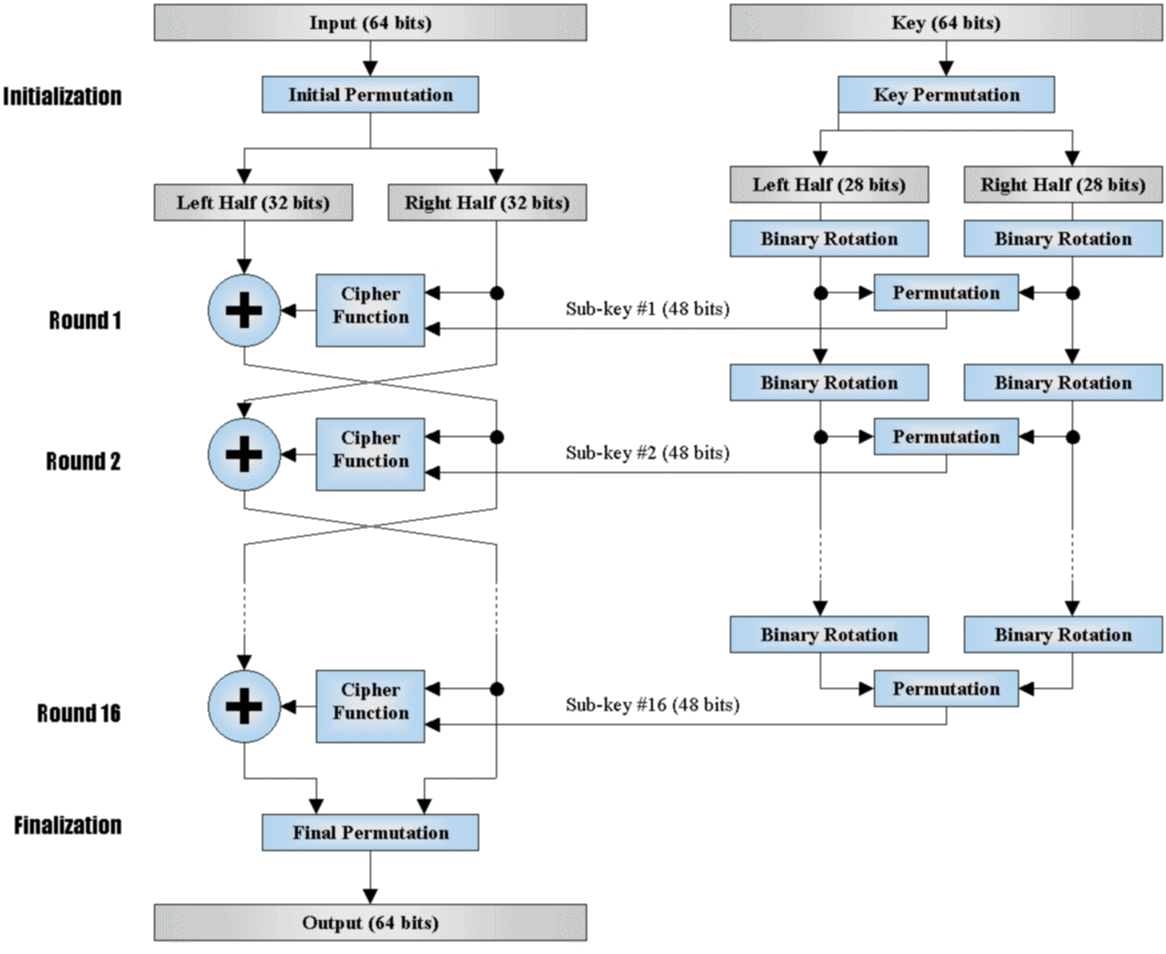
\includegraphics[scale=0.4]{des_algo.png}
\caption{The DES Algorithm. The plus sign indicates an XOR.}
\label{fig_des_algo}
\end{center}
\end{figure*}

\subsection{AES Algorithm}

AES is substantially more complicated. No joke. Just check out this 
comic strip explaining it:

\begin{itemize}
\item
\url{http://www.moserware.com/2009/09/stick-figure-guide-to-advanced.html}
\end{itemize}

Yeah. It's bananas. But it works. Ok, it's not THAT bad, but it IS 
sensitive to multiple side-channel attacks: malevolent manipulation of CPU
cache, and timing-based attacks are two examples. There are effective counter-
measures to them, but they're tricky.

You can get a general picture of the algorithm by looking at 
Figure~\ref{fig_aes_algo}. Each of the blocks --SubBytes, ShiftRows,
MixColumns, and AddRoundKey-- require their own explanation that may be found
in later figures. TBD TBD TBD.

\begin{figure*}
\begin{center}
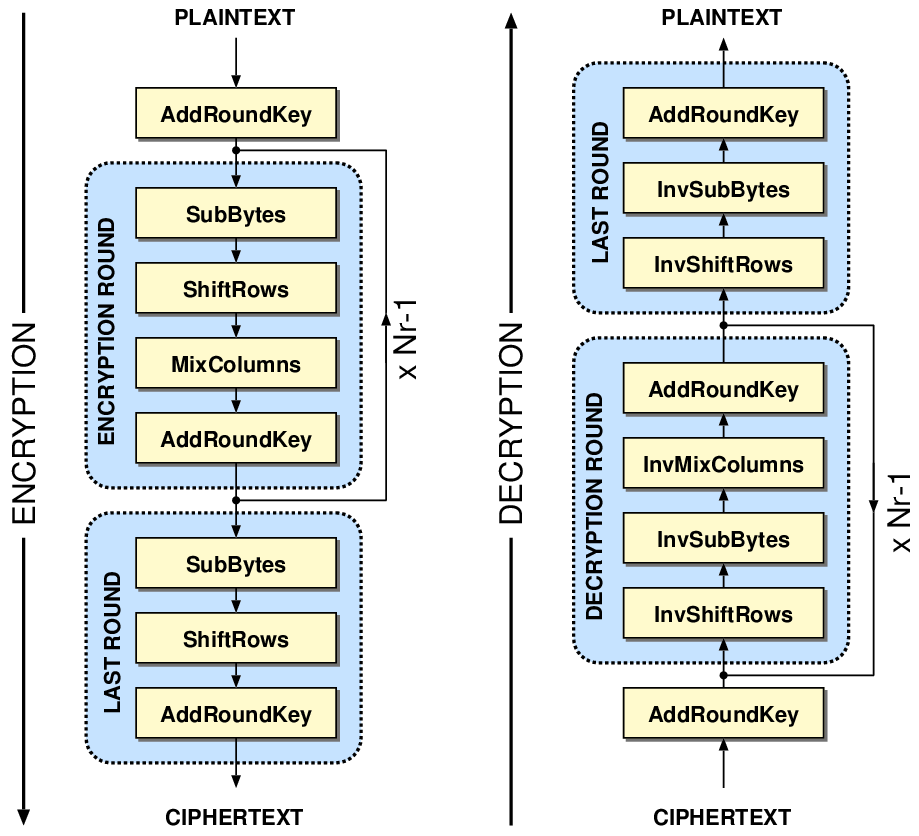
\includegraphics[scale=0.4]{aes_algo.png}
\caption{The AES Algorithm.}
\label{fig_aes_algo}
\end{center}
\end{figure*}

\section{Summary and Approach}

\IEEEPARstart{A}{fter} covering the basics of the algorithm, each paper then
describes how their particular FPGA can implement state machines, and how this
affects the design choices they made.

\section{Major Contributions}

\IEEEPARstart{A} simple introduction to pipelining with practical applications.

%\begin{tabular}{|c|c|c|c|}
%\hline
%Value & Expected & Measured & \% error \\
%\hline
%$\omega_{o}$ (Hz) & 5894 & 2747 & -53.4\\
%\hline
%phase (deg) & 45 & 41.096 & -8.67\\
%\hline
%\end{tabular}

\section{Analysis and Improvements}

\IEEEPARstart{Y}{ou} know, without their source code, I can't make any
meaningful analysis or improvements.

\section{Shortcomings}

\IEEEPARstart{W}{here} is the source code? It isn't in the paper itself and
isn't referenced to exist anywhere else! A block diagram is nice, but please:
source code so we can replicate your work!

This is what I'm talking about:

\begin{quote}
Various implementations are presented in various
platforms for DES algorithm in [1], [3], [4], [9], [10].
However the design provided in this study is implemented
in Virtex6 FPGA. In the current pipelined design, we put
buffers in input and output stages of each round. The key
scheduler part does quite a novel task in current
implementation. It floods the sub keys to appropriate round.
The key scheduler implementation specifications are as
follow: 
\end{quote}

If I can't replicate your work, then it's not science, and I can't trust 
any results you give me.

\section{Conclusion}

\IEEEPARstart{G}{ood} god. Please stop screen-shotting non-free software
waveform viewers. Stop screen-shotting period! And please, PLEASE make the
source code and raw data available and easy to find!

Seriously.

\bibliographystyle{IEEEtran}
\bibliography{des-paper,aes-paper}

\end{document}
